\documentclass[12pt,a4paper]{article}
\usepackage[slovene]{babel}
\usepackage[utf8]{inputenc}
\usepackage{amsmath}
\usepackage{graphicx}
\begin{document}

\setlength{\parskip}{1em}
\setlength{\parindent}{0pt}

\tableofcontents

\section{Teoretični del}

\subsection{Uvod}

V javnem sektorju, za razliko od zasebnega sektorja, profitabilnost
ni tako zelo pomembna. Pogosto njeno vlogo zamenja učinkovitost. 
Učinkovitost je stopnja pri kateri je zagotavljanje storitev maksimizirana pri omejenih 
virih. Včasih je merjena tudi obratno -- kot stopnja, pri kateri je uporaba virov 
minimizirana pri pogoju zadostne zagotovitve storitev. \cite{Lovell2002}

Javni sektor je pogosto obravnavan kot neučinkovit zaradi odsotnosti
tekmovanja na trgu. Pričakovanja nam pravijo, da v primeru, ko obstajata
javna in privatna storitev, bo javna manj učinkovita. To razmišljanje tudi
spodbuja gibanja v smer privatizacije javnih storitev v številnih državah.
Vendar je pomembno omeniti, da pogosto ne primerjamo primerljivih
storitev med javnim in zasebnim sektorjem. Namreč 
pogosto država zagotavlja blago in storitve tam, kjer je trg odpovedal.
\cite{Lovell2002}

Številne študije so pokazale, da tako organizacije iz tako javnega
kot tudi zasebnega sektorja ne uporabljajo svojih omejenih virov
učinkovito. Možna posledica je, da bi prerazporeditev virov iz
zagotavljanja blaga in storitev, ki imajo razmeroma nizke
mejne družbene koristi, k tistim z razmeroma visokimi mejnimi
družbenimi koristmi, izboljšala splošno družbeno blaginjo.
Druga posledica je, da viri niso bili uporabljeni na najbolj 
produktiven način; to pomeni, da je mogoče proizvesti več
blaga in storitev brez dodatnih virov. \cite{Yaisawarng2002}

\subsection{Konceptno ogrodje}

Vladne agencije običajno vključujejo več enot za izvajanje 
storitev, ki zagotavljajo ,,prvovrstne'' socialne storitve. 
Primer za Avstralijo lahko vidimo na sliki 
\ref{fig:government_structure}.


\begin{figure}[htbp]
    \centering
    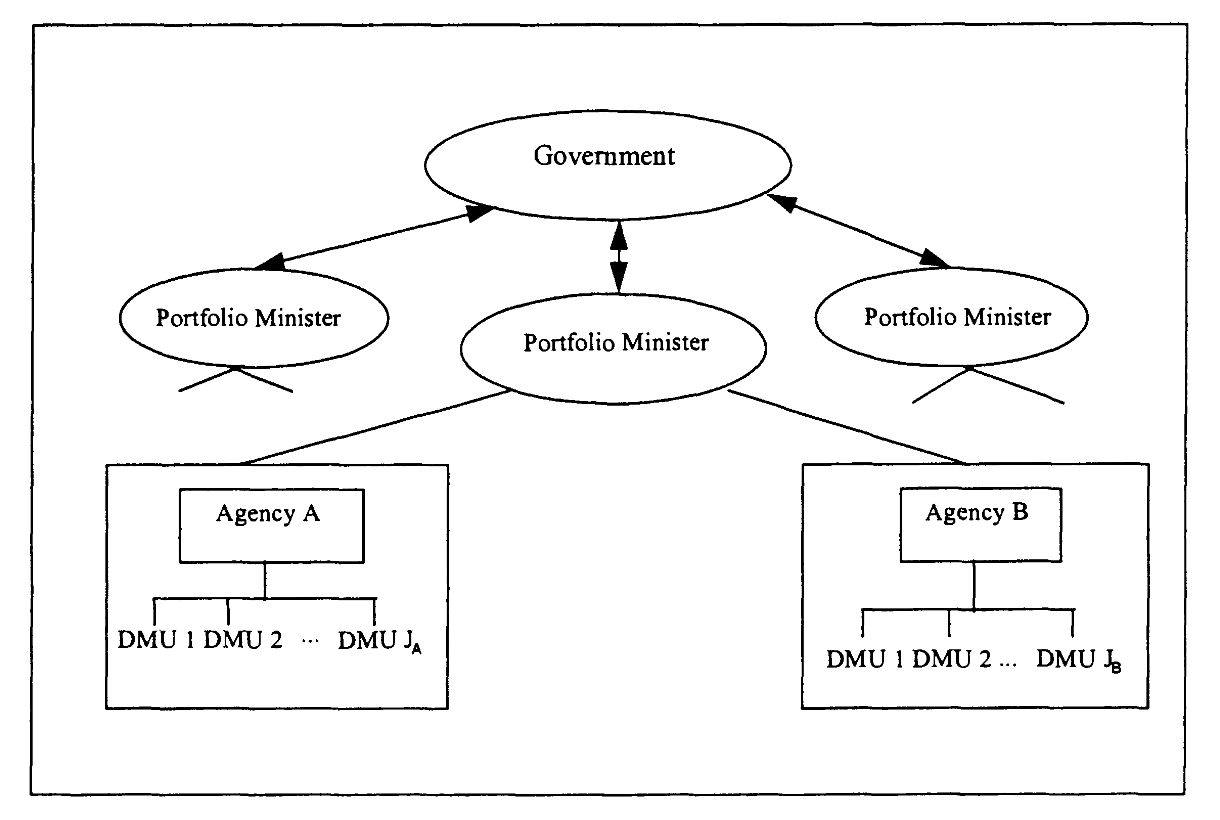
\includegraphics[width=0.7\textwidth]{government_structure.png}
    \caption{Struktura agencij v splošnem vladnem sektorju}
    \label{fig:government_structure}
\end{figure}

Agenciji $A$ in $B$ sta odgovorni za zagotavljanje vladnih storitev, 
na primer ministrstvo za šolstvo (osnovno in srednješolsko 
izobraževanje) ter ministrstvo za delo (poklicno izobraževanje).
Agencija A vključuje $J_A$ osnovnih in srednjih šol, Agencija B 
pa $J_B$ izobraževalnih centrov. Delovanje teh agencij nadzoruje
pristojni minister. \cite{Yaisawarng2002}

Vlade lahko zagotavljajo osnovne socialne storitve na področjih
zdravstva, izobraževanja in varnosti. Te storitve se financirajo
iz državenga proračuna (ki se financira iz davkov ter državenga
dolga) in ne prek zaračunavanja storitev. 

\subsection{DEA}

Analiza podatkovne ovojnice (angl.\ data envelopment analysis -- DEA) je 
metoda linearnega programiranja, ki ustvari proizvodno mejo iz 
najproduktivnejših opazovanj v vzorcu. Ta meja predstavlja 
dejansko najboljšo prakso v naboru vključenih enot odločanja
(DMU) in ne le teoretičnega optimuma. Ocena učinkovitosti 
vsake opazovane enote se izračuna glede na to mejo najboljše 
prakse. Ta postopek nam omogoča primerjavo uspešnosti različnih
enot, ki izvajajo podobne naloge, z najboljšimi izvajalci
v vzorcu. \cite{Yaisawarng2002}

Indeks učinkovitosti DEA je sestavljena mera uspešnosti,
ki upošteva vse vhodne in izhodne podatke v modelu ter služi
kot dopolnilno orodje k obstoječim meram produktivnosti,
kot npr.\ proizvod na delavca. Ocena učinkovitosti DEA
kaže delež trenutnih vložkov, ki
bi jih enota uporabila, če bi bila produktivno učinkovita,
ter nakazuje, ali se lahko določen vložek dodatno zmanjša brez
zmanjšanja drugih vložkov pri dani ravni izhodni vrednosti,
obenem pa zagotavlja nabor uteži, ki se uporabljajo za
oblikovanje ciljne točke za neučinkovito enoto. \cite{Yaisawarng2002}


\begin{figure}[htbp]
    \centering
    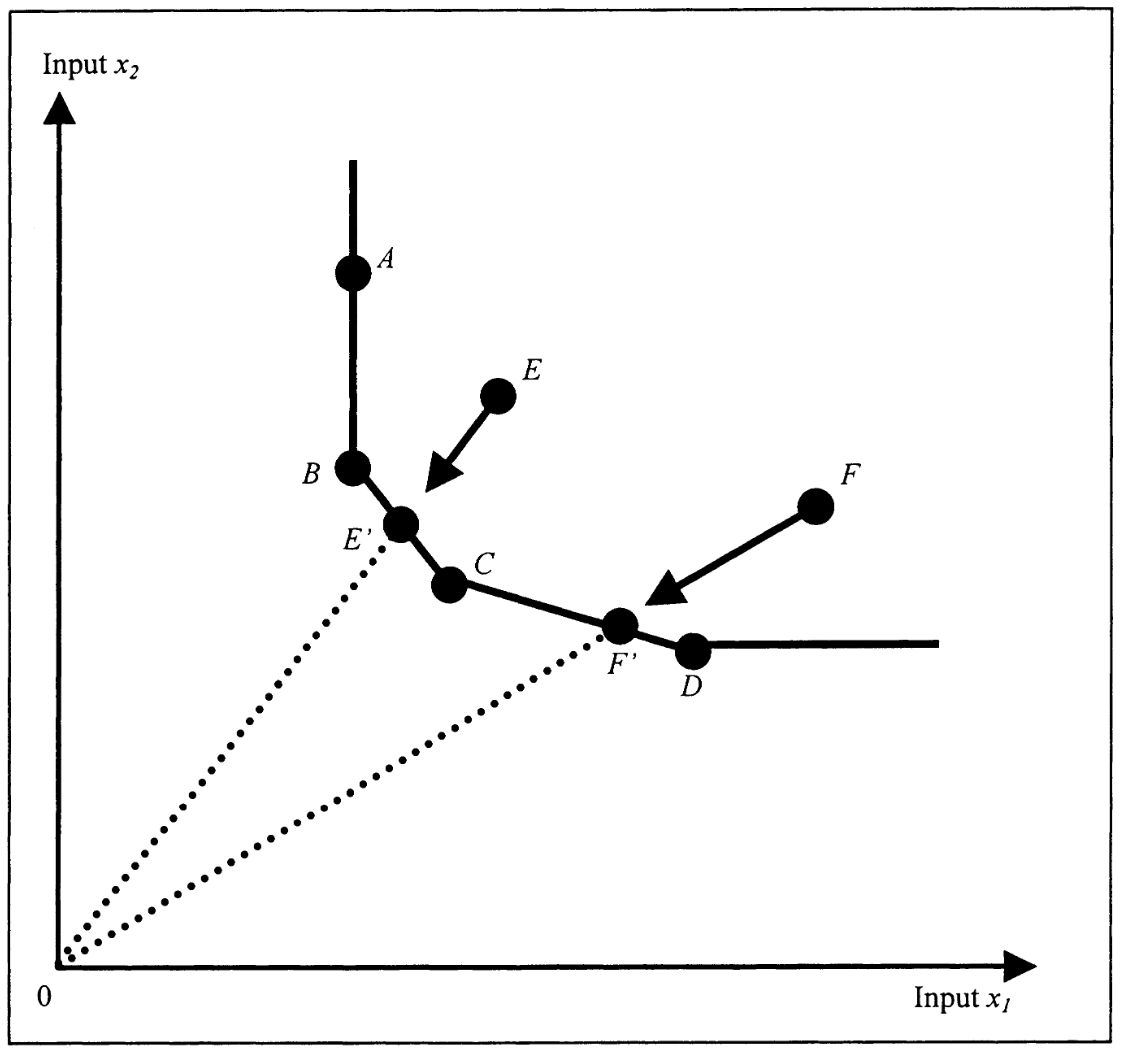
\includegraphics[width=0.7\textwidth]{dea_frontier.png}
    \caption{Proizvodna meja DEA}
    \label{fig:dea_frontier}
\end{figure}

Slika \ref{fig:dea_frontier} predstavlja učinkovitost pri 
varčevanju z vložki za agencijo, sestavljeno iz šestih
DMU-jev, od $A$ do $F$. Vsak DMU proizvede enako količino
proizvoda $y$ pri uporabi različnih količin $x_1$ in $x_2$.
Za neučinkovit DMU $F$ velja $0F' < 0F$, oz.\ $0F'/0F < 1$,
kajti $F'$ je bližje izhodišču kot $F$. Če $F$ postane 
učinkovit, ob ohranitvi enakega razmerja vložkov, bo
na točki $F'$. Primera učinkovitih DMU-jev pa sta $C$
in $D$, ki imata višje razmerje med $y$ in $x_1$ ter
$x_2$.

V tem primeru bi moral vodja neučinkovitega DMU-ja uporabiti
rezultate DEA kot vodilo pri razvoju načrta za izboljšanje
učinkovitosti. Postopek se začne z notranjo preiskavo DMU
za identifikacijo možnih razlag za prekomerno uporabo vložkov.
Ta lahko identificira situacije, ki so specifične za ta DMU
in so zunaj nadzora vodje. V tem primeru se morajo te situacije
izvzeti iz DEA modela. Navedli bomo postopek, kako se DEA
lahko uporabi za izboljšanje učinkovitosti.

\begin{enumerate}
    \item Uporabimo ocene učinkovitosti DEA in tako poiščemo
    vse neučinkovite DMU-je in obseg potencialnih izboljšav. 
    Identificiramo tudi učinkovite DMU-je, primerne za 
    primerjavo in specifična področja za preiskavo.
    
    \item Izvedemo preiskavo neučinkovitega 
    DMU-ja, da lahko določimo vzroke prekomerne 
    uporabe vložkov.
    
    \item Posvetujemo se z primerljivimi učinkovitimi DMU-ji
    o njihovih koristnih praksah.
    
    \item Analiziramo kvalitativne in kvantitativne informacije
    iz preiskave in upoštevamo uteži primerjalnih enot DEA.
    
    \item Oblikujemo strateški načrt za implementacijo v 
    neučinkovitem DMU-ju. To lahko zahteva prestrukturiranje 
    organizacije in spremembe v upravljanju.
\end{enumerate}


\bibliographystyle{plain}
\bibliography{javni_sektor}

\end{document}
